% thios section describes the computational image complexity analysis

The theory framework section meticulously examined the architectural evolution, revealing a recurring cycle oscillating between complex and simple styles.
Given the recent technological advancements and contemporary architectural trends, there is a compelling indication that the present era is poised for a shift toward complexity, countering the preceding Modernist movement characterized by minimalism and simplicity.

In pursuit of validating this hypothesis, we conceived a ``Computational Image Complexity Analysis'' system.
The primary goal was to empirically validate the insights gleaned from our theoretical analysis, which indicated a trend towards architectural complexity.
This system assigns complexity scores to the most emblematic buildings representing various architectural styles and historical eras.

The computational image complexity analysis module is a Python script that assesses complexity by quantifying the number of elements within a building's design.
The higher the count of elements, the higher the assigned complexity score, and vice versa.
This approach draws inspiration from Venturi et al.'s reflection on complexity, as articulated in their work\cite{Venturi1977}.
They posited that a building's complexity could be gauged by the time it takes to mentally process and form a coherent image of its constituent elements.
This fundamental concept underpins the computational image complexity analysis module's methodology(Figure\ref{fig:ImageComplexityAnalysisFlowchart}).

%% Figure Methodology flowchart
    \begin{figure}[!htb]
      \centering
      % trim=left 190 down 250 right 150 top5
      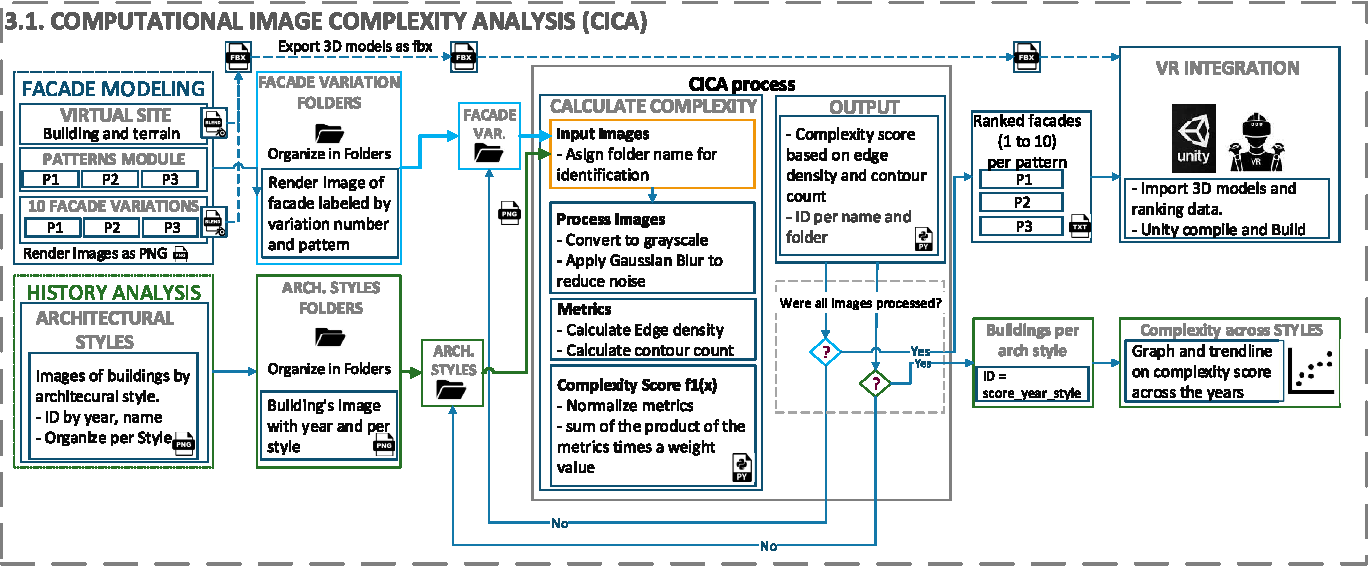
\includegraphics[width= \linewidth, trim=0 0 0 0, clip]{Images/ImageComplexityAnalysisFlowchart}
      \caption{Flowchart illustrating the applications of Computational Image Complexity Analysis, including its role in analyzing complexity scores for historical architectural styles and ranking modeled facades for the VR Building Complexity System.}
      \label{fig:ImageComplexityAnalysisFlowchart}
    \end{figure}

The Computational Image Complexity Analysis systems as shown in Figure\ref{fig:ImageComplexityAnalysisFlowchart} works by using building images as input, it then processes the image to increase contrast and reduce noise to improve element recognition.
Then it determines the number of elements by edge density, since an accentuated edge can be correlated to a new element of the building then it can be extrapolated that higher the edge density the more complex the building would be interpreted on this script as separation hence another element.

Edge density is calculated by applying Canny Edge Detection\cite{OpenCV2023}, a multi stage algorithm used to detect edges in an image by dividing the number of non-zero (edge) pixels in the edges image by the total number of pixels in the image \ref{fig:CannyEdgePlotHistory}.

%%Figure Canny Edge of historic buildings
     \begin{figure}[htb]
          \centering
          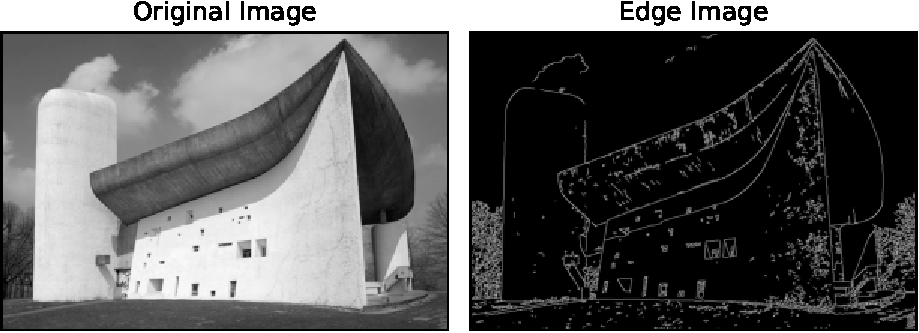
\includegraphics[width= \linewidth]{Images/CannyEdgePlotHistory}
          \caption{Original image of Chapelle Notre-Dame-du-Haut de Ronchamp, built in 1955 (left) next to the pos Canny edge processing plot by OpenCV reflecting edge density of building (right).}
          \label{fig:CannyEdgePlotHistory}
        \end{figure}

The Computational image complexity analysis system was also used for selecting the 10 level of complexity variations for the experiment (Figure \ref{fig:CannyEdgePlotRender})

%%Figure Canny Edge of render buildings
     \begin{figure}[htb]
          \centering
          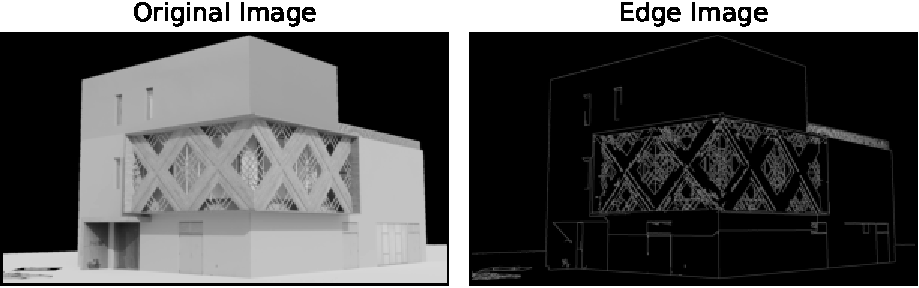
\includegraphics[width= \linewidth]{Images/CannyEdgePlotRender}
          \caption{Original render of facades variation modeled in blender for the VR complexity analysis system used on this research (left) next to the pos Canny edge processing plot by OpenCV reflecting edge density of render (right).}
          \label{fig:CannyEdgePlotRender}
        \end{figure}

